\documentclass[a4paper,10pt]{article}
\setlength{\parindent}{0.5cm}
\setlength{\parskip}{\baselineskip} 

\usepackage{graphicx}
\usepackage[utf8]{inputenc}
\usepackage[spanish]{babel}
\usepackage{color}
\usepackage{placeins}
\usepackage[T1]{fontenc}
\usepackage{listings}

\lstset{ %
language=C++,                % choose the language of the code
basicstyle=\footnotesize,       % the size of the fonts that are used for the code
numbers=left,                   % where to put the line-numbers
numberstyle=\footnotesize,      % the size of the fonts that are used for the line-numbers
stepnumber=1,                   % the step between two line-numbers. If it is 1 each line will be numbered
numbersep=5pt,                  % how far the line-numbers are from the code
backgroundcolor=\color{white},  % choose the background color. You must add \usepackage{color}
showspaces=false,               % show spaces adding particular underscores
showstringspaces=false,         % underline spaces within strings
showtabs=false,                 % show tabs within strings adding particular underscores
frame=single,           % adds a frame around the code
tabsize=2,          % sets default tabsize to 2 spaces
captionpos=b,           % sets the caption-position to bottom
breaklines=true,        % sets automatic line breaking
breakatwhitespace=false,    % sets if automatic breaks should only happen at whitespace
escapeinside={\%*}{*)}          % if you want to add a comment within your code
}

% Creates indexes for Table of Contents, List of Figures, List of Tables and Index
\makeindex


\title{

\includegraphics[width=0.25\textwidth]{content/escudodelauba2uj.jpg}

\includegraphics[width=0.35\textwidth]{content/logofiubabajatm9.jpg}\\[2.5ex] 
\textbf{66:20 Organizaci\'on de Computadoras  
    Trabajo Pr\'actico 0: Infraestructura B\'asica
}
}

\author{
	\textbf{Profesor Titular:} \\ 
	Dr. Ing. Jos\'e Luis Hamkalo  \\[2.5ex] 
	\textbf{Docentes:} \\
	Ing. Leandro Santi  \\
	Ing. Hern\'an P\'erez Masci\\
    Ing. Luciano Natale\\[2.5ex]
	\textbf{Alumnos:}								\\ 
	Petalás, Alexis \textit{Padr\'on Nro. 86742}\\
    Opromolla, Giovanni \textit{Padr\'on Nro. 87761}				\\
    Tapia, Jimena Soledad \textit{Padr\'on Nro. 88392}				\\[2.5ex]
	\normalsize{2do. Cuatrimestre de 2015}									\\
	\normalsize{66.20 Organizaci\'on de Computadoras  $-$ Pr\'actica Martes}	\\
	\normalsize{Facultad de Ingenier\'ia, Universidad de Buenos Aires}		\\   
}
\date{}

\begin{document}

	\maketitle

\thispagestyle{empty}   % quita el número en la primer página

\begin{abstract}
Con el presente trabajo pr\'actico logramos familiarizarnos con las herramientas a utilizar a lo largo del cuatrimestre para resolver los trabajos propuestos por la c\'atedra; en particular con el entorno de desarrollo que emula una m\'aquina MIPS corriendo una versi\'on reciente del sistema operativo NetBSD.

\end{abstract}

\newpage

%
\renewcommand{\contentsname}{Indice}
\tableofcontents
\addtocontents{toc}{\par\nobreak \mbox{}\hfill{\bf P\'ag.}\par\nobreak}

\newpage

\section{Introducci\'on}
Se va a desarrollar un programa en lenguaje C que permita multiplicar matrices de n\'umeros en punto flotante de doble precisi\'on. Dichas matrices a multiplicar ingresan por entrada est\'andar y el resultado de la multiplicaci\'on tomadas de a pares se muestra por salida est\'andar (stdout).

\subsection{Objetivo}
Implementar una funci\'on multiplicadora de matrices que sea portable al menos en NetBSD (usando el simulador GXemul [1]) y la versi\'on de Linux (Knoppix, RedHat, Debian, Ubuntu) usada para correr el simulador, Linux/i386.

\newpage

\section{An\'alisis del Problema}
Se detalla a continuaci\'on el an\'alisis previo a la resoluci\'on del trabajo pr\'actico, clasificado en temas de inter\'es:

\subsection{Situaci\'on inicial del equipo}
\begin{enumerate}
\item La tecnolog\'ia a utilizar es nueva para los integrantes del equipo.
\item Se requiere la configuraci\'on y preparaci\'on de un entorno de desarrollo espec\'ifico. Tambi\'en nuevo para los integrantes del equipo.
\item El lenguaje solicitado para programar la soluci\'on no es de uso diario de los integrantes del equipo.
\end{enumerate}

De este an\'alisis se resolvi\'o inicialmente focalizarse en el setup del ambiente y luego en el desarrollo propio del trabajo pr\'actico.

\subsection{Problem\'atica a Resolver}
\begin{enumerate}
\item Las matrices de entrada pueden estar mal formadas o incompletas, es decir, pueden contener menos cantidad de valores de los esperados por la dimensi\'on definida.
\item La cantidad de matrices de entrada puede no ser par, interrumpiendo el procesamiento normal de datos ya que el mismo pretende ir multiplicando las matrices de a pares.
\item Las dimensiones indicadas pueden tener un formato incorrecto.
\item Las dimensiones de un par de matrices de entrada, o par formado por la matriz resultante del par anterior, pueden ser incompatibles para su multiplicaci\'on.
\item Si el valor en una posici\'on de la matriz es una letra o cualquier caracter no casteable a un número, se considera como un 0.
\end{enumerate}

De este an\'alisis se extrajeron consideraciones para la construcci\'on del parser y el manejo de errores.

\newpage

\section{Diseño e implementaci\'on del programa}


\subsection{Implementaci\'on del programa}

A partir del problema propuesto, se busc\'o desarrollar una soluci\'on que fuera efic\'az y sencilla, centr\'andose en la reutilizaci\'on de esta soluci\'on como c\'odigo de entrada para el desarrollo de funciones en MIPS32 en pr\'oximos trabajos pr\'acticos. \par

Se separ\'o la l\'ogica de parseo de comandos de entrada y la de c\'alculo de multiplicaci\'on de las matrices.\par


\subsection{Esquema de diseño}
A continuación se muestra un diagrama simplificado de las relaciones de los header de problema propuesto.

\begin{figure}[htbp]
	    \centering
		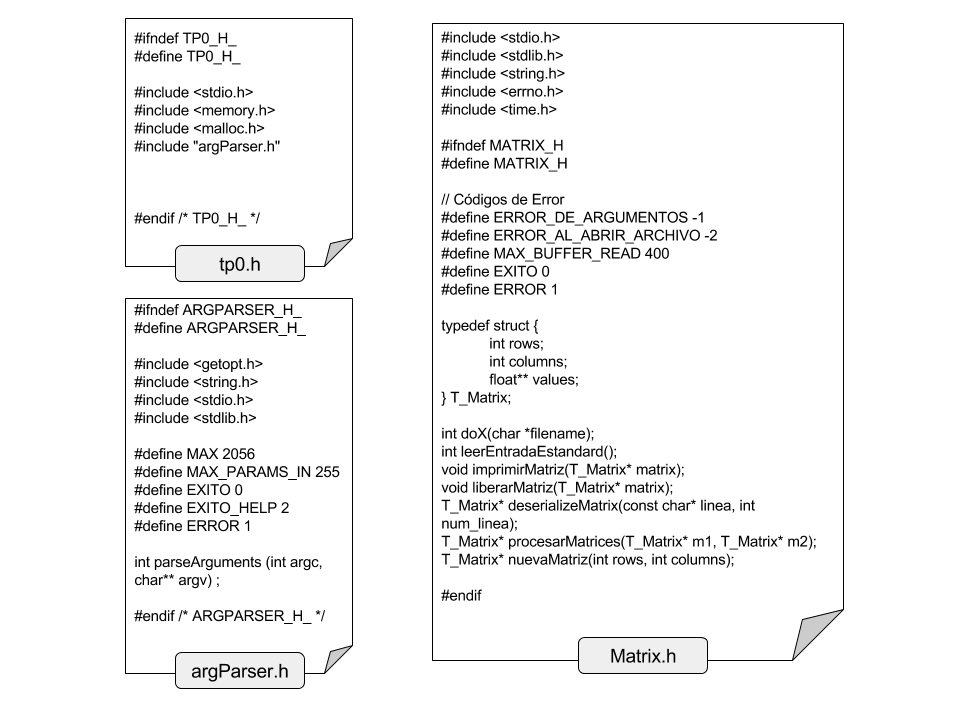
\includegraphics[width=0.90\textwidth]{content/diagrama_h.png}
	    \caption{\scriptsize{Diagrama interfaces.}}
	    \label{fig002}
      \end{figure}

\newpage

Y las relaciones de uso entre las mismas.

\begin{figure}[htbp]
	    \centering
		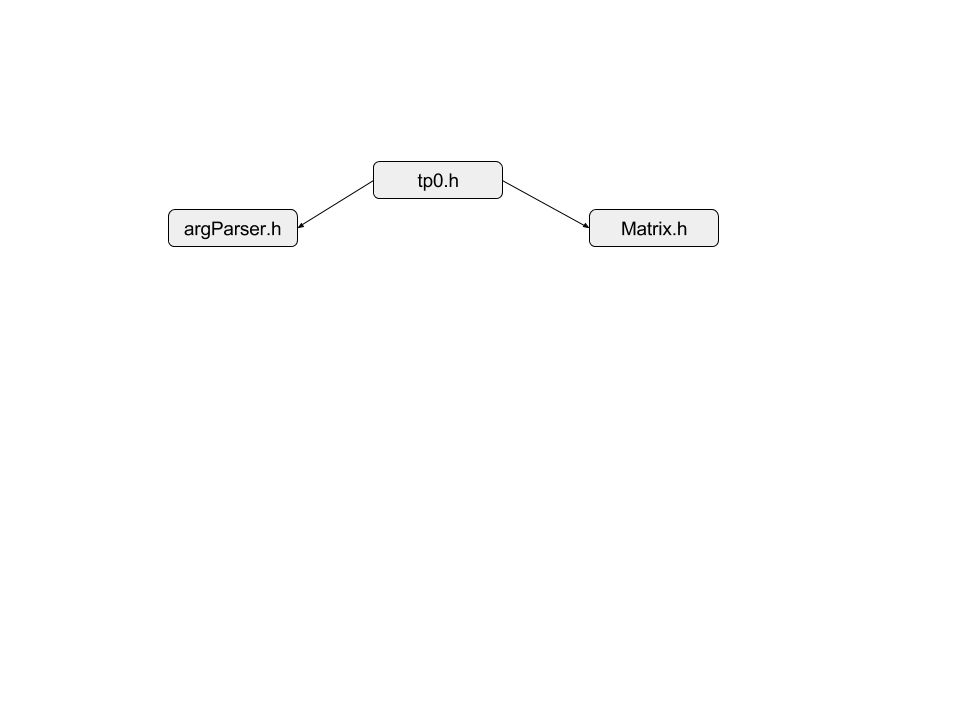
\includegraphics[width=0.90\textwidth]{content/DiagramaRelaciones.png}
	    \caption{\scriptsize{Diagrama Relaciones.}}
	    \label{fig002}
      \end{figure}

\newpage


\section{Compilaci\'on y ejecuci\'on}

Para la compilaci\'on del programa se implement\'o un Makefile como se puede  ver a continuaci\'on:
\\
\begin{lstlisting}[numbers=left,language=bash]
DEPS = \
       src/argParser.h \
       src/Matrix.h \
       src/tp0.h

OBJ = build/obj/argParser.o \
      build/obj/Matrix.o \
      build/obj/tp0.o

VIRTUAL = gxemul-6620-20070927

CC=gcc
CP=cp
CFLAGS=-I./src -Wall $(ACFLAGS)

build: prepare tp0

tp0: $(OBJ)
	gcc -o build/$@ $(OBJ) $(CFLAGS)

build/obj/argParser.o: src/argParser.c $(DEPS)
	$(CC) -c -o $@ src/argParser.c $(CFLAGS)

build/obj/Matrix.o: src/Matrix.c $(DEPS)
	$(CC) -c -o $@ src/Matrix.c $(CFLAGS)
	
build/obj/tp0.o: src/tp0.c $(DEPS)
	$(CC) -c -o $@ src/tp0.c $(CFLAGS)

prepare:
	-mkdir -p build
	-mkdir -p build/doc
	-mkdir -p build/obj

clean:
	rm -rf build tags

virtual-start:
	sudo ifconfig lo:0 172.20.0.1
	if [ ! -d ./gxemul/$(VIRTUAL) ]; then bzip2 -dc ./gxemul/$(VIRTUAL).tar.bz2 | cpio --sparse -i -v; mv $(VIRTUAL) ./gxemul/ ; fi
	echo "ssh -f -N -R 2222:127.0.0.1:22 $(USER)@172.20.0.1" | xclip -sel clip
	./gxemul/$(VIRTUAL)/gxemul -e 3max -d ./gxemul/$(VIRTUAL)/netbsd-pmax.img

virtual-reset:
	rm -rf ./gxemul/$(VIRTUAL)

virtual-authkey:
	cat ~/.ssh/id_rsa.pub | ssh -p 2222 root@127.0.0.1 "rm -rf .ssh/authorized_keys; mkdir -p ~/.ssh; cat >> ~/.ssh/authorized_keys"

virtual-deploy:
	ssh -p 2222 root@127.0.0.1 "rm -rf ~/deploy; mkdir -p ~/deploy;"
	scp -P 2222 -r makefile src data root@127.0.0.1:/root/deploy

doc: prepare
	pandoc README.md -o build/doc/README.pdf
	pdflatex --output-directory build/doc docs/informe.tex
	pdflatex --output-directory build/doc docs/informe.tex
	pdflatex --output-directory build/doc docs/informe.tex

doc-preview: doc
	evince build/doc/informe.pdf &

doc-spell:
	aspell -t check docs/informe.tex -d es

export: doc
	tar -czvf build/entrega_tp0.tar.gz makefile src data -C build/doc/ informe.pdf README.pdf

\end{lstlisting}


Para compilar el programa utilizando el Makefile se deben seguir los pasos que se indican en el archivo Readme del proyecto: \\
\begin{lstlisting}[numbers=left,language=bash]
Pasos para correr en la virtual:
$ make virtual-start
login: root
pass: orga6620

Ctrl+Shift+V o copy-paste de la linea "ssh -f -N -R 2222:127.0.0.1:22 giovanni@172.20.0.1"

abrir otra consola y hacer un:
$ make virtual-deploy (despliega los archivos importarntes a la virtual)

ahora volvemos a la consolita anterior y entran en deploy
$ cd deploy/
$ make build
Ahi se les compila todo en MIPS... 

el ejecutable se genera en ~/deploy/build/tp0
los archivos para correr estan bajo la carpeta de data/

Ejemplo de corrida: ~/deploy/$ build/tp0 < data/in1.txt
\end{lstlisting}
\newpage

\section{Pruebas}

Para probar la aplicaci\'on se ejecutaron las pruebas sencillas presentadas a modo de ejemplo en el enunciado del trabajo. \\

\subsection{-h Help}

\begin{lstlisting}[numbers=left,language=bash]
  $ build/tp0 -h
Usage:
  ./tp0 -h
  ./tp0 -V
  ./tp0  < in_file > out_file
Options:
  -V, --version	Print version and quit.
  -h, --help	Print this information and quit.
Examples:
  ./tp0 < in.txt > out.txt
  cat in.txt | ./tp0 > out.txt

\end{lstlisting}



\subsection{-V Version}


\begin{lstlisting}[numbers=left,language=bash]
	$ build/tp0 -V

	TP0 - Infraestructura Basica
  (66.20) Organizacion de las Computadoras
------------------------------------------------
	2do Cuatrimestre de 2015
	      Version: 1.0

Autores:
         Petalas, Alexis - 86742
         Opromolla, Giovanni - 87761
         Tapia, Jimena Soledad - 88392

\end{lstlisting}


\subsection{build/tp0 < data/in1.txt}
Se realiza una prueba simple, con un archivo que contiene un conjunto de matrices cuyas dimensiones son compatibles para la multiplicaci\'on de a pares. Se muestra el archivo de entrada y el resultado de la ejecuci\'on:

\begin{lstlisting}[numbers=left,language=bash]
2x3 1 2 3 4 5 6.1
3x2 1 0 0 0 0 1
3x3 1 2 3 4 5 6.1 3 2 1
3x1 1 1 0
\end{lstlisting}
\begin{lstlisting}
$ build/tp0 < data/in1.txt
2x2 1.000000 3.000000 4.000000 6.100000 
3x1 3.000000 9.000000 5.000000
\end{lstlisting}

\subsection{build/tp0 < data/in2.txt}
Se realiza una prueba con un archivo que contiene un conjunto de matrices cuyas dimensiones no son compatibles para la multiplicaci\'on de a pares. Se muestra el archivo de entrada y el resultado de la ejecuci\'on:

\begin{lstlisting}[numbers=left,language=bash]
2x2 1 3 4 6.1
3x1 3 9 5
\end{lstlisting}
\begin{lstlisting}
$ build/tp0 < data/in2.txt
Las propiedades de multiplicacion de matrices no estan satisfechas.
\end{lstlisting}


\subsection{build/tp0 < data/in3.txt}
Se realiza una prueba con un archivo que contiene datos con formato incorrecto. No se respeta el formato de entrada acordado "NxM a1,1 a1,2 ... a1,M a2,1 a2,2 ... a2,M ... aN,1 aN,2 ... aN,M". Se muestra el archivo de entrada y el resultado de la ejecuci\'on:

\begin{lstlisting}[numbers=left,language=bash]
12xx 12351
\end{lstlisting}
\begin{lstlisting}
$ build/tp0 < data/in3.txt
Error al leer los valores de NxM en la linea 0.
\end{lstlisting}

\subsection{build/tp0 < data/in4.txt}
Se realiza una prueba con un archivo que contiene matrices incompletas, es decir, que las dimensiones indicadas no se corresponden con los valores aX,Y listados. Se muestra el archivo de entrada donde se esperan 6 valores y el resultado de la ejecuci\'on:

\begin{lstlisting}[numbers=left,language=bash]
2x2 1.1 2.2 3.3
\end{lstlisting}
\begin{lstlisting}
$ build/tp0 < data/in4.txt
Faltan valores en la matriz de 2x2 de la linea 0.
\end{lstlisting}

\newpage

\section{Manejo de errores}
Para manejar errores y advertirle al usuario de los mismos se utilizaron mensajes por linea de comando:\\

\subsection{Comando inexistente}
En este caso se eligió mostrar el menú de opciones para que el usuario pueda seleccionar un comando correcto, dentro de los entendidos por el programa.

\begin{lstlisting}[language=bash]
$ build/tp0 -u

build/tp0: invalid option -- 'u'
Usage:
  ./tp0 -h
  ./tp0 -V
  ./tp0  < in_file > out_file
Options:
  -V, --version	Print version and quit.
  -h, --help	Print this information and quit.
Examples:
  ./tp0 < in.txt > out.txt
  cat in.txt | ./tp0 > out.txt
  
\end{lstlisting}
\newpage


\section{Conclusiones}
Luego del desarrollo realizado, logramos familiarizarnos con las herramientas a utilizar a lo largo del cuatrimestre, dejamos el entorno de desarrollo que emula la m\'aquina MIPS funcional y listo para los pr\'oximos trabajos pr\'acticos de la materia.


\newpage

\section{C\'odigo}


\subsection{C\'odigo C}
\title{argParser.h}
\begin{lstlisting}[language=C]

#ifndef ARGPARSER_H_
#define ARGPARSER_H_

#include <getopt.h>
#include <string.h>
#include <stdio.h>
#include <stdlib.h>

#define MAX 2056
#define MAX_PARAMS_IN 255
#define EXITO 0
#define EXITO_HELP 2
#define ERROR 1

int parseArguments (int argc, char** argv) ;

#endif /* ARGPARSER_H_ */

\end{lstlisting}

\title{argParser.c}
\begin{lstlisting}[language=C]

#include "argParser.h"

int showMenuHelp()
{
    printf("Usage:\n");
    printf("  ./tp0 -h\n");
    printf("  ./tp0 -V\n");
    printf("  ./tp0  < in_file > out_file\n");
    printf("Options:\n");
    printf("  -V, --version\tPrint version and quit.\n");
    printf("  -h, --help\tPrint this information and quit.\n");
    printf("Examples:\n");
    printf("  ./tp0 < in.txt > out.txt\n");
    printf("  cat in.txt | ./tp0 > out.txt\n");
    return EXITO;
}

int showMenuVersion()
{
	printf("\n\tTP0 - Infraestructura Basica\n");
	printf("  (66.20) Organizacion de las Computadoras\n");
 	printf("------------------------------------------------\n");
	printf("\t2do Cuatrimestre de 2015\n");
	printf("\t      Version: 1.0\n");
	printf("\nAutores:\n");
	printf("         Petalas, Alexis - 86742\n");
	printf("         Opromolla, Giovanni - 87761\n");
	printf("         Tapia, Jimena Soledad - 88392\n\n");
	return EXITO;

}


int readOptions (int argc, char** argv, const char* op_cortas, const struct option op_largas[]) {

	int siguiente_opcion = 0;
	int result = ERROR;

	siguiente_opcion = getopt_long(argc, argv, op_cortas, op_largas, NULL);

	switch (siguiente_opcion) {
		case 'h' : /* -h o --help */
			showMenuHelp();
			result = EXITO_HELP;
			break;
		case 'V' : /* -V o --version */
			showMenuVersion();
			result = EXITO_HELP;
			break;
		case '?' : /* opcion no valida */
			showMenuHelp();
			result = EXITO_HELP;
			break;
		default : /* Algo mas? No esperado. Abortamos */
			result = EXITO;
	}

	return result;
}



int parseArguments (int argc, char** argv) {
  
	int result = ERROR;
		
	/* Una cadena que lista las opciones cortas validas */
	const char* op_cortas = "hV" ;

	/* Una estructura de varios arrays describiendo los valores largos */
	const struct option op_largas[] = {
		{ "help",         0,  NULL,   'h'},
		{ "version",      0,  NULL,   'V'},
		{ NULL,           0,  NULL,   0  }
	};

	result = readOptions(argc, argv, op_cortas, op_largas);
	
	if(result == ERROR){
	    showMenuHelp();
	}
	
	return result;
}

\end{lstlisting}

\title{Matrix.h}
\begin{lstlisting}[language=C]
#include <stdio.h>
#include <stdlib.h>
#include <string.h>
#include <errno.h>
#include <time.h>

#ifndef MATRIX_H
#define MATRIX_H

// Codigos de Error
#define ERROR_DE_ARGUMENTOS -1
#define ERROR_AL_ABRIR_ARCHIVO -2
#define MAX_BUFFER_READ 400
#define EXITO 0
#define ERROR 1

typedef struct {
	int rows;
	int columns;
	float** values;
} T_Matrix;

int doX(char *filename);
int leerEntradaEstandard();
void imprimirMatriz(T_Matrix* matrix);
void liberarMatriz(T_Matrix* matrix);
T_Matrix* deserializeMatrix(const char* linea, int num_linea);
T_Matrix* procesarMatrices(T_Matrix* m1, T_Matrix* m2);
T_Matrix* nuevaMatriz(int rows, int columns);

#endif

\end{lstlisting}
\title{Matrix.c
\begin{lstlisting}[language=C]

#include "Matrix.h"

#define BUF_SIZE 255

int leerEntradaEstandard()
{

    char line[BUF_SIZE];
    int num_linea = 0;

    T_Matrix* m1 = NULL;
    T_Matrix* m2 = NULL;
    T_Matrix* m_resultado = NULL;
    /** Lectura de stdin para obtener las matrices linea por linea **/

    while((fgets(line,BUF_SIZE,stdin)) != NULL){

    	if(strlen(line) > 2){
			if (num_linea%2 == 0)		/** Pares **/
			{
				m1 = deserializeMatrix(line, num_linea);
				if (m1 == NULL) {
          /** Algun problema surgio al deserealizar la matriz **/
          fprintf(stderr, "Ocurrio un error al procesar una las lineas. Verique el formato y la cantidad de matrices en el archivo.\n");
  				break;
        }
			}
			else						/** Impares **/
			{
				m2 = deserializeMatrix(line, num_linea);
				if (m2 == NULL){
				  liberarMatriz(m1);
          fprintf(stderr, "Ocurrio un error al procesar una las lineas. Verique el formato y la cantidad de matrices en el archivo.\n");
          break;
        } 	/** Algun problema surgio al deserealizar la matriz **/
				else{
					m_resultado = procesarMatrices(m1, m2);

					if(m_resultado != NULL)
						imprimirMatriz(m_resultado);

					liberarMatriz(m1);
					liberarMatriz(m2);
					liberarMatriz(m_resultado);
				}
			}
			++num_linea;
    	}
	}

    return EXITO;
}

void imprimirMatriz(T_Matrix* matrix){
	int row, columns;
  printf("%dx%d ", matrix->rows, matrix->columns);
	for (row=0; row<matrix->rows; row++)
	{
	    for(columns=0; columns<matrix->columns; columns++)
	         printf("%f ", matrix->values[row][columns]);
	}
  printf("\n");
}

void liberarMatriz(T_Matrix* matrix){

	int row;

	for( row=0; row<matrix->rows; row++ ) {
	    free( matrix->values[row] );
	}
	free( matrix->values );

	free(matrix);
	matrix = NULL;
}


char* serializeMatrix(T_Matrix* m ){
    char* matrix_str = NULL;

    return matrix_str;
}

T_Matrix* deserializeMatrix(const char* linea, int num_linea){

	int rows = -1;
	int columns = -1;
	int val = sscanf(linea, "%dx%d", &rows, &columns);

	/** Verificar que se hayan podido leer ambos valores **/
	if (val != 2)
	{
		fprintf(stderr, "Error al leer los valores de NxM en la linea %d.\n", num_linea);
		exit(1);
	}
	/** Verificar que ambos valores sean mayores a cero **/
	if((rows < 0) || (columns < 0)){
		fprintf(stderr, "Los valres de NxM deben ser valores positivos. Linea conflictiva: %d.\n", num_linea);
		exit(1);
	}

	/** Creo matriz y aloco su memoria **/
	T_Matrix* matrix = nuevaMatriz(rows, columns);

	/** Obtengo los valores de la matriz **/
    char* valores = strstr (linea," ");;
    char *token;
    token = strtok(valores, " ");

    int f=0, c=0;
    while( (token != NULL) && (f < rows ) )
    {
    	matrix->values[f][c] = atof(token);
    	token = strtok(NULL, " ");
    	if(f < rows){
    		c++;
    		if(c == columns){
    			f++;
    			c = 0;
    		}
    	}
    }

    /** Matriz incompleta **/
    if(f != rows){
    	fprintf(stderr, "Faltan valores en la matriz de %dx%d de la linea %d.\n", matrix->rows, matrix->columns, num_linea );
    	liberarMatriz(matrix);
    	exit(1);
    }

    /** Imprimo la matriz **/
    //imprimirMatriz(matrix);

	return matrix;
}

T_Matrix* nuevaMatriz(int rows, int columns){

	T_Matrix* matrix = (T_Matrix*) malloc(sizeof (T_Matrix) );

	matrix->rows = rows;
	matrix->columns = columns;

	/** Aloco espacio para la matriz **/
	matrix->values = (float**) malloc (sizeof(float*)*matrix->rows);
	int i = 0;
	for(; i < matrix->rows; ++i){
		matrix->values[i] = (float*) malloc (sizeof(float)*matrix->columns);
	}

	return matrix;
}

T_Matrix* procesarMatrices(T_Matrix* m1, T_Matrix* m2){

	T_Matrix* matrix = NULL;

	if(m1->columns == m2->rows){

		/** Creo matriz y aloco su memoria **/
		matrix = nuevaMatriz(m1->rows, m2->columns);

		int row1, column2,  k;
		float sum;

	    for(row1=0; row1<m1->rows; ++row1) //filas de la primer matriz
	    {
	    	for(column2=0; column2<m2->columns; ++column2)  //columnas de la segunda matriz
	    	{
	    		sum=0;

	    		for(k=0;k<m1->columns;k++)
	    			sum=sum + m1->values[row1][k] * m2->values[k][column2];

	    		matrix->values[row1][column2]=sum;
	    	}
	    }

	}else{
    	fprintf(stderr, "Las propiedades de multiplicacion de matrices no estan satisfechas.\n");
    	exit(1);
	}

	return matrix;

}

\end{lstlisting}


\title{tp0.h}
\begin{lstlisting}[language=C]
/*
 * tp0.h
 *
 *  Created on: Sep 9, 2015
 *      Author: giovanni
 */

#ifndef TP0_H_
#define TP0_H_

#include <stdio.h>
#include <memory.h>
#include <malloc.h>
#include "argParser.h"



#endif /* TP0_H_ */

\end{lstlisting}

\title{tp0.c}
\begin{lstlisting}[language=C]
#include "tp0.h"
#include "Matrix.h"

int main(int argc, char** argv){
	
      int result = parseArguments(argc, argv);
            
      if(result == 0)
	  result = leerEntradaEstandard();
      else if (result == 1)
	  perror("Error al obtener los argumentos.");
            
      return 0;
}
\end{lstlisting}

\subsection{C\'odigo MIPS}
\title{Porci\'on de c\'odigo ilustrativa - argParser.o}
\begin{lstlisting}

argParser.o:     file format elf32-tradlittlemips

Disassembly of section .text:

00000000 <showMenuHelp>:
   0:	3c1c0000 	lui	gp,0x0
   4:	279c0000 	addiu	gp,gp,0
   8:	0399e021 	addu	gp,gp,t9
   c:	27bdffd8 	addiu	sp,sp,-40
  10:	afbc0010 	sw	gp,16(sp)
  14:	afbf0020 	sw	ra,32(sp)
  18:	afbe001c 	sw	s8,28(sp)
  1c:	afbc0018 	sw	gp,24(sp)
  20:	03a0f021 	move	s8,sp
  24:	8f840000 	lw	a0,0(gp)
  28:	00000000 	nop
  2c:	24840000 	addiu	a0,a0,0
  30:	8f990000 	lw	t9,0(gp)
  34:	00000000 	nop
  38:	0320f809 	jalr	t9
  3c:	00000000 	nop
  40:	8fdc0010 	lw	gp,16(s8)
  44:	00000000 	nop
  48:	8f840000 	lw	a0,0(gp)
  4c:	00000000 	nop
  50:	24840008 	addiu	a0,a0,8
  54:	8f990000 	lw	t9,0(gp)
  58:	00000000 	nop
  5c:	0320f809 	jalr	t9
  60:	00000000 	nop
  64:	8fdc0010 	lw	gp,16(s8)
  68:	00000000 	nop
  6c:	8f840000 	lw	a0,0(gp)
  70:	00000000 	nop
  74:	24840014 	addiu	a0,a0,20
  78:	8f990000 	lw	t9,0(gp)
  7c:	00000000 	nop
  80:	0320f809 	jalr	t9
  84:	00000000 	nop
  88:	8fdc0010 	lw	gp,16(s8)

\end{lstlisting}

\title{Porci\'on de c\'odigo ilustrativa - Matrix.o}
\begin{lstlisting}

Matrix.o:     file format elf32-tradlittlemips

Disassembly of section .text:

00000000 <leerEntradaEstandard>:
   0:	3c1c0000 	lui	gp,0x0
   4:	279c0000 	addiu	gp,gp,0
   8:	0399e021 	addu	gp,gp,t9
   c:	27bdfec8 	addiu	sp,sp,-312
  10:	afbc0010 	sw	gp,16(sp)
  14:	afbf0130 	sw	ra,304(sp)
  18:	afbe012c 	sw	s8,300(sp)
  1c:	afbc0128 	sw	gp,296(sp)
  20:	03a0f021 	move	s8,sp
  24:	afc00118 	sw	zero,280(s8)
  28:	afc0011c 	sw	zero,284(s8)
  2c:	afc00120 	sw	zero,288(s8)
  30:	afc00124 	sw	zero,292(s8)
  34:	27c40018 	addiu	a0,s8,24
  38:	240500ff 	li	a1,255
  3c:	8f860000 	lw	a2,0(gp)
  40:	8f990000 	lw	t9,0(gp)
  44:	00000000 	nop
  48:	0320f809 	jalr	t9
  4c:	00000000 	nop
  50:	8fdc0010 	lw	gp,16(s8)
  54:	14400003 	bnez	v0,64 <leerEntradaEstandard+0x64>
  58:	00000000 	nop
  5c:	10000071 	b	224 <leerEntradaEstandard+0x224>
  60:	00000000 	nop
  64:	27c40018 	addiu	a0,s8,24
  68:	8f990000 	lw	t9,0(gp)
  6c:	00000000 	nop
  70:	0320f809 	jalr	t9
  74:	00000000 	nop
  78:	8fdc0010 	lw	gp,16(s8)
  7c:	2c420003 	sltiu	v0,v0,3
  80:	1440ffec 	bnez	v0,34 <leerEntradaEstandard+0x34>
  84:	00000000 	nop
  88:	8fc20118 	lw	v0,280(s8)

\end{lstlisting}

\title{Porci\'on de c\'odigo ilustrativa - tp0.o}
\begin{lstlisting}

tp0.o:     file format elf32-tradlittlemips

Disassembly of section .text:

00000000 <main>:
   0:	3c1c0000 	lui	gp,0x0
   4:	279c0000 	addiu	gp,gp,0
   8:	0399e021 	addu	gp,gp,t9
   c:	27bdffd0 	addiu	sp,sp,-48
  10:	afbc0010 	sw	gp,16(sp)
  14:	afbf0028 	sw	ra,40(sp)
  18:	afbe0024 	sw	s8,36(sp)
  1c:	afbc0020 	sw	gp,32(sp)
  20:	03a0f021 	move	s8,sp
  24:	afc40030 	sw	a0,48(s8)
  28:	afc50034 	sw	a1,52(s8)
  2c:	8fc40030 	lw	a0,48(s8)
  30:	8fc50034 	lw	a1,52(s8)
  34:	8f990000 	lw	t9,0(gp)
  38:	00000000 	nop
  3c:	0320f809 	jalr	t9
  40:	00000000 	nop
  44:	8fdc0010 	lw	gp,16(s8)
  48:	afc20018 	sw	v0,24(s8)
  4c:	8fc20018 	lw	v0,24(s8)
  50:	00000000 	nop
  54:	14400008 	bnez	v0,78 <main+0x78>
  58:	00000000 	nop
  5c:	8f990000 	lw	t9,0(gp)
  60:	00000000 	nop
  64:	0320f809 	jalr	t9
  68:	00000000 	nop
  6c:	8fdc0010 	lw	gp,16(s8)
  70:	1000000d 	b	a8 <main+0xa8>
  74:	afc20018 	sw	v0,24(s8)
  78:	8fc30018 	lw	v1,24(s8)
  7c:	24020001 	li	v0,1
  80:	14620009 	bne	v1,v0,a8 <main+0xa8>
  84:	00000000 	nop
  88:	8f840000 	lw	a0,0(gp)

\end{lstlisting}

\newpage
\begin{thebibliography}{99}
\bibitem {gxemul} GXemul,http://gavare.se/gxemul/.
\bibitem {The NetBSD project} The NetBSD project, http://www.netbsd.org/.
\bibitem {time } time man page http://unixhelp.ed.ac.uk/CGI/man-cgi?time.
\bibitem {GNU} GNU gprof http://www.cs.utah.edu/dept/old/texinfo/as/gprof.html.
\end{thebibliography}
\end{document}

